% Options for packages loaded elsewhere
\PassOptionsToPackage{unicode}{hyperref}
\PassOptionsToPackage{hyphens}{url}
\PassOptionsToPackage{dvipsnames,svgnames,x11names}{xcolor}
%
\documentclass[
  letterpaper,
  DIV=11,
  numbers=noendperiod]{scrartcl}

\usepackage{amsmath,amssymb}
\usepackage{iftex}
\ifPDFTeX
  \usepackage[T1]{fontenc}
  \usepackage[utf8]{inputenc}
  \usepackage{textcomp} % provide euro and other symbols
\else % if luatex or xetex
  \usepackage{unicode-math}
  \defaultfontfeatures{Scale=MatchLowercase}
  \defaultfontfeatures[\rmfamily]{Ligatures=TeX,Scale=1}
\fi
\usepackage{lmodern}
\ifPDFTeX\else  
    % xetex/luatex font selection
\fi
% Use upquote if available, for straight quotes in verbatim environments
\IfFileExists{upquote.sty}{\usepackage{upquote}}{}
\IfFileExists{microtype.sty}{% use microtype if available
  \usepackage[]{microtype}
  \UseMicrotypeSet[protrusion]{basicmath} % disable protrusion for tt fonts
}{}
\makeatletter
\@ifundefined{KOMAClassName}{% if non-KOMA class
  \IfFileExists{parskip.sty}{%
    \usepackage{parskip}
  }{% else
    \setlength{\parindent}{0pt}
    \setlength{\parskip}{6pt plus 2pt minus 1pt}}
}{% if KOMA class
  \KOMAoptions{parskip=half}}
\makeatother
\usepackage{xcolor}
\setlength{\emergencystretch}{3em} % prevent overfull lines
\setcounter{secnumdepth}{-\maxdimen} % remove section numbering
% Make \paragraph and \subparagraph free-standing
\ifx\paragraph\undefined\else
  \let\oldparagraph\paragraph
  \renewcommand{\paragraph}[1]{\oldparagraph{#1}\mbox{}}
\fi
\ifx\subparagraph\undefined\else
  \let\oldsubparagraph\subparagraph
  \renewcommand{\subparagraph}[1]{\oldsubparagraph{#1}\mbox{}}
\fi

\usepackage{color}
\usepackage{fancyvrb}
\newcommand{\VerbBar}{|}
\newcommand{\VERB}{\Verb[commandchars=\\\{\}]}
\DefineVerbatimEnvironment{Highlighting}{Verbatim}{commandchars=\\\{\}}
% Add ',fontsize=\small' for more characters per line
\usepackage{framed}
\definecolor{shadecolor}{RGB}{241,243,245}
\newenvironment{Shaded}{\begin{snugshade}}{\end{snugshade}}
\newcommand{\AlertTok}[1]{\textcolor[rgb]{0.68,0.00,0.00}{#1}}
\newcommand{\AnnotationTok}[1]{\textcolor[rgb]{0.37,0.37,0.37}{#1}}
\newcommand{\AttributeTok}[1]{\textcolor[rgb]{0.40,0.45,0.13}{#1}}
\newcommand{\BaseNTok}[1]{\textcolor[rgb]{0.68,0.00,0.00}{#1}}
\newcommand{\BuiltInTok}[1]{\textcolor[rgb]{0.00,0.23,0.31}{#1}}
\newcommand{\CharTok}[1]{\textcolor[rgb]{0.13,0.47,0.30}{#1}}
\newcommand{\CommentTok}[1]{\textcolor[rgb]{0.37,0.37,0.37}{#1}}
\newcommand{\CommentVarTok}[1]{\textcolor[rgb]{0.37,0.37,0.37}{\textit{#1}}}
\newcommand{\ConstantTok}[1]{\textcolor[rgb]{0.56,0.35,0.01}{#1}}
\newcommand{\ControlFlowTok}[1]{\textcolor[rgb]{0.00,0.23,0.31}{#1}}
\newcommand{\DataTypeTok}[1]{\textcolor[rgb]{0.68,0.00,0.00}{#1}}
\newcommand{\DecValTok}[1]{\textcolor[rgb]{0.68,0.00,0.00}{#1}}
\newcommand{\DocumentationTok}[1]{\textcolor[rgb]{0.37,0.37,0.37}{\textit{#1}}}
\newcommand{\ErrorTok}[1]{\textcolor[rgb]{0.68,0.00,0.00}{#1}}
\newcommand{\ExtensionTok}[1]{\textcolor[rgb]{0.00,0.23,0.31}{#1}}
\newcommand{\FloatTok}[1]{\textcolor[rgb]{0.68,0.00,0.00}{#1}}
\newcommand{\FunctionTok}[1]{\textcolor[rgb]{0.28,0.35,0.67}{#1}}
\newcommand{\ImportTok}[1]{\textcolor[rgb]{0.00,0.46,0.62}{#1}}
\newcommand{\InformationTok}[1]{\textcolor[rgb]{0.37,0.37,0.37}{#1}}
\newcommand{\KeywordTok}[1]{\textcolor[rgb]{0.00,0.23,0.31}{#1}}
\newcommand{\NormalTok}[1]{\textcolor[rgb]{0.00,0.23,0.31}{#1}}
\newcommand{\OperatorTok}[1]{\textcolor[rgb]{0.37,0.37,0.37}{#1}}
\newcommand{\OtherTok}[1]{\textcolor[rgb]{0.00,0.23,0.31}{#1}}
\newcommand{\PreprocessorTok}[1]{\textcolor[rgb]{0.68,0.00,0.00}{#1}}
\newcommand{\RegionMarkerTok}[1]{\textcolor[rgb]{0.00,0.23,0.31}{#1}}
\newcommand{\SpecialCharTok}[1]{\textcolor[rgb]{0.37,0.37,0.37}{#1}}
\newcommand{\SpecialStringTok}[1]{\textcolor[rgb]{0.13,0.47,0.30}{#1}}
\newcommand{\StringTok}[1]{\textcolor[rgb]{0.13,0.47,0.30}{#1}}
\newcommand{\VariableTok}[1]{\textcolor[rgb]{0.07,0.07,0.07}{#1}}
\newcommand{\VerbatimStringTok}[1]{\textcolor[rgb]{0.13,0.47,0.30}{#1}}
\newcommand{\WarningTok}[1]{\textcolor[rgb]{0.37,0.37,0.37}{\textit{#1}}}

\providecommand{\tightlist}{%
  \setlength{\itemsep}{0pt}\setlength{\parskip}{0pt}}\usepackage{longtable,booktabs,array}
\usepackage{calc} % for calculating minipage widths
% Correct order of tables after \paragraph or \subparagraph
\usepackage{etoolbox}
\makeatletter
\patchcmd\longtable{\par}{\if@noskipsec\mbox{}\fi\par}{}{}
\makeatother
% Allow footnotes in longtable head/foot
\IfFileExists{footnotehyper.sty}{\usepackage{footnotehyper}}{\usepackage{footnote}}
\makesavenoteenv{longtable}
\usepackage{graphicx}
\makeatletter
\def\maxwidth{\ifdim\Gin@nat@width>\linewidth\linewidth\else\Gin@nat@width\fi}
\def\maxheight{\ifdim\Gin@nat@height>\textheight\textheight\else\Gin@nat@height\fi}
\makeatother
% Scale images if necessary, so that they will not overflow the page
% margins by default, and it is still possible to overwrite the defaults
% using explicit options in \includegraphics[width, height, ...]{}
\setkeys{Gin}{width=\maxwidth,height=\maxheight,keepaspectratio}
% Set default figure placement to htbp
\makeatletter
\def\fps@figure{htbp}
\makeatother

\KOMAoption{captions}{tableheading}
\makeatletter
\makeatother
\makeatletter
\makeatother
\makeatletter
\@ifpackageloaded{caption}{}{\usepackage{caption}}
\AtBeginDocument{%
\ifdefined\contentsname
  \renewcommand*\contentsname{Table of contents}
\else
  \newcommand\contentsname{Table of contents}
\fi
\ifdefined\listfigurename
  \renewcommand*\listfigurename{List of Figures}
\else
  \newcommand\listfigurename{List of Figures}
\fi
\ifdefined\listtablename
  \renewcommand*\listtablename{List of Tables}
\else
  \newcommand\listtablename{List of Tables}
\fi
\ifdefined\figurename
  \renewcommand*\figurename{Figure}
\else
  \newcommand\figurename{Figure}
\fi
\ifdefined\tablename
  \renewcommand*\tablename{Table}
\else
  \newcommand\tablename{Table}
\fi
}
\@ifpackageloaded{float}{}{\usepackage{float}}
\floatstyle{ruled}
\@ifundefined{c@chapter}{\newfloat{codelisting}{h}{lop}}{\newfloat{codelisting}{h}{lop}[chapter]}
\floatname{codelisting}{Listing}
\newcommand*\listoflistings{\listof{codelisting}{List of Listings}}
\makeatother
\makeatletter
\@ifpackageloaded{caption}{}{\usepackage{caption}}
\@ifpackageloaded{subcaption}{}{\usepackage{subcaption}}
\makeatother
\makeatletter
\@ifpackageloaded{tcolorbox}{}{\usepackage[skins,breakable]{tcolorbox}}
\makeatother
\makeatletter
\@ifundefined{shadecolor}{\definecolor{shadecolor}{rgb}{.97, .97, .97}}
\makeatother
\makeatletter
\makeatother
\makeatletter
\makeatother
\ifLuaTeX
  \usepackage{selnolig}  % disable illegal ligatures
\fi
\IfFileExists{bookmark.sty}{\usepackage{bookmark}}{\usepackage{hyperref}}
\IfFileExists{xurl.sty}{\usepackage{xurl}}{} % add URL line breaks if available
\urlstyle{same} % disable monospaced font for URLs
\hypersetup{
  pdftitle={ISC\_6153\_Assignment\_2},
  pdfauthor={Sophia Costa \& James Sturges},
  colorlinks=true,
  linkcolor={blue},
  filecolor={Maroon},
  citecolor={Blue},
  urlcolor={Blue},
  pdfcreator={LaTeX via pandoc}}

\title{ISC\_6153\_Assignment\_2}
\author{Sophia Costa \& James Sturges}
\date{}

\begin{document}
\maketitle
\ifdefined\Shaded\renewenvironment{Shaded}{\begin{tcolorbox}[breakable, interior hidden, frame hidden, boxrule=0pt, enhanced, borderline west={3pt}{0pt}{shadecolor}, sharp corners]}{\end{tcolorbox}}\fi

\hypertarget{isc-6153-assignment-2}{%
\subsection{ISC 6153 Assignment 2}\label{isc-6153-assignment-2}}

Use the online NOAA climate index time series calculator (see link
below) to generate a time series of yearly PDSI values for Northeast
Arizona for the period of 1895-2021. Export the time series to CSV file
in order to provide quantitative answers.

{[}\url{https://www.ncdc.noaa.gov/cag/divisional/time-series}, under
divisional{]}

\hypertarget{formatting}{%
\subsection{Formatting}\label{formatting}}

\#reads in monthly PDSI values for Northeast Arizona 1895-2021 and
formats date times

\begin{Shaded}
\begin{Highlighting}[]
\NormalTok{NE\_AZ\_PDSI }\OtherTok{=} \FunctionTok{read\_csv}\NormalTok{(}\StringTok{"data/NE\_AZ\_PDSI\_1895{-}2021.csv"}\NormalTok{)}

\NormalTok{NE\_AZ\_PDSI }\OtherTok{=}\NormalTok{ NE\_AZ\_PDSI }\SpecialCharTok{\%\textgreater{}\%} 
  \FunctionTok{mutate}\NormalTok{(}\AttributeTok{Date =} \FunctionTok{ym}\NormalTok{(Date))}

\NormalTok{NE\_AZ\_PDSI }\OtherTok{=}\NormalTok{ NE\_AZ\_PDSI }\SpecialCharTok{\%\textgreater{}\%} 
  \FunctionTok{mutate}\NormalTok{(}\AttributeTok{year =} \FunctionTok{year}\NormalTok{(Date),}
         \AttributeTok{month =} \FunctionTok{month}\NormalTok{(Date),}
         \AttributeTok{day =} \FunctionTok{day}\NormalTok{(Date))}
\end{Highlighting}
\end{Shaded}

\hypertarget{questions}{%
\subsection{Questions}\label{questions}}

\textbf{(1a)} How many months and equivalent years (months/12) did
Northeast Arizona experience dry conditions (PDSI \textless{} 0) and how
many wet conditions (PDSI \textgreater0). What is the ratio between dry
to wet months?

\begin{Shaded}
\begin{Highlighting}[]
\NormalTok{dry\_mons }\OtherTok{=}\NormalTok{ NE\_AZ\_PDSI }\SpecialCharTok{\%\textgreater{}\%} 
  \FunctionTok{filter}\NormalTok{(Value }\SpecialCharTok{\textless{}} \DecValTok{0}\NormalTok{) }\SpecialCharTok{\%\textgreater{}\%} 
  \FunctionTok{nrow}\NormalTok{()}

\NormalTok{dry\_years }\OtherTok{=}\NormalTok{ NE\_AZ\_PDSI }\SpecialCharTok{\%\textgreater{}\%} 
  \FunctionTok{group\_by}\NormalTok{(year) }\SpecialCharTok{\%\textgreater{}\%}
  \FunctionTok{summarize}\NormalTok{(}\AttributeTok{count =} \FunctionTok{as.numeric}\NormalTok{(}\FunctionTok{any}\NormalTok{(Value }\SpecialCharTok{\textless{}} \DecValTok{0}\NormalTok{))) }\SpecialCharTok{\%\textgreater{}\%}
  \FunctionTok{summarize}\NormalTok{(}\AttributeTok{count\_of\_years =} \FunctionTok{sum}\NormalTok{(count)) }\SpecialCharTok{\%\textgreater{}\%} 
  \FunctionTok{pull}\NormalTok{(count\_of\_years)}

\NormalTok{wet\_mons }\OtherTok{=}\NormalTok{ NE\_AZ\_PDSI }\SpecialCharTok{\%\textgreater{}\%} 
  \FunctionTok{filter}\NormalTok{(Value }\SpecialCharTok{\textgreater{}} \DecValTok{0}\NormalTok{) }\SpecialCharTok{\%\textgreater{}\%} 
  \FunctionTok{nrow}\NormalTok{()}

\NormalTok{wet\_years }\OtherTok{=}\NormalTok{ NE\_AZ\_PDSI }\SpecialCharTok{\%\textgreater{}\%} 
  \FunctionTok{group\_by}\NormalTok{(year) }\SpecialCharTok{\%\textgreater{}\%}
  \FunctionTok{summarize}\NormalTok{(}\AttributeTok{count =} \FunctionTok{as.numeric}\NormalTok{(}\FunctionTok{any}\NormalTok{(Value }\SpecialCharTok{\textgreater{}} \DecValTok{0}\NormalTok{))) }\SpecialCharTok{\%\textgreater{}\%}
  \FunctionTok{summarize}\NormalTok{(}\AttributeTok{count\_of\_years =} \FunctionTok{sum}\NormalTok{(count)) }\SpecialCharTok{\%\textgreater{}\%} 
  \FunctionTok{pull}\NormalTok{(count\_of\_years)}

\NormalTok{dry\_wet\_mons\_ratio }\OtherTok{=}\NormalTok{ dry\_mons}\SpecialCharTok{/}\NormalTok{wet\_mons}
\end{Highlighting}
\end{Shaded}

\textbf{Answers Q1a}

\begin{Shaded}
\begin{Highlighting}[]
\NormalTok{dry\_mons}
\end{Highlighting}
\end{Shaded}

\begin{verbatim}
[1] 890
\end{verbatim}

\begin{Shaded}
\begin{Highlighting}[]
\NormalTok{dry\_years}
\end{Highlighting}
\end{Shaded}

\begin{verbatim}
[1] 111
\end{verbatim}

\begin{Shaded}
\begin{Highlighting}[]
\NormalTok{wet\_mons}
\end{Highlighting}
\end{Shaded}

\begin{verbatim}
[1] 634
\end{verbatim}

\begin{Shaded}
\begin{Highlighting}[]
\NormalTok{wet\_years}
\end{Highlighting}
\end{Shaded}

\begin{verbatim}
[1] 93
\end{verbatim}

\begin{Shaded}
\begin{Highlighting}[]
\NormalTok{dry\_wet\_mons\_ratio}
\end{Highlighting}
\end{Shaded}

\begin{verbatim}
[1] 1.403785
\end{verbatim}

{[}10 points{]}

\textbf{(1b)} How many months and equivalent years did Northeast Arizona
experienced severe drought conditions (PDSI \textless{} -3) and how many
extreme conditions (PDSI \textless{} -4)?

\begin{Shaded}
\begin{Highlighting}[]
\NormalTok{severe\_mons }\OtherTok{=}\NormalTok{ NE\_AZ\_PDSI }\SpecialCharTok{\%\textgreater{}\%} 
  \FunctionTok{filter}\NormalTok{(Value }\SpecialCharTok{\textless{}=} \SpecialCharTok{{-}}\DecValTok{3}\NormalTok{) }\SpecialCharTok{\%\textgreater{}\%}
  \FunctionTok{nrow}\NormalTok{()}

\NormalTok{severe\_years }\OtherTok{=}\NormalTok{ NE\_AZ\_PDSI }\SpecialCharTok{\%\textgreater{}\%} 
  \FunctionTok{group\_by}\NormalTok{(year) }\SpecialCharTok{\%\textgreater{}\%}
  \FunctionTok{summarize}\NormalTok{(}\AttributeTok{count =} \FunctionTok{as.numeric}\NormalTok{(}\FunctionTok{any}\NormalTok{(Value }\SpecialCharTok{\textless{}=} \SpecialCharTok{{-}}\DecValTok{4}\NormalTok{))) }\SpecialCharTok{\%\textgreater{}\%}
  \FunctionTok{summarize}\NormalTok{(}\AttributeTok{count\_of\_years =} \FunctionTok{sum}\NormalTok{(count)) }\SpecialCharTok{\%\textgreater{}\%} 
  \FunctionTok{pull}\NormalTok{(count\_of\_years)}


\NormalTok{extreme\_mons }\OtherTok{=}\NormalTok{ NE\_AZ\_PDSI }\SpecialCharTok{\%\textgreater{}\%} 
  \FunctionTok{filter}\NormalTok{(Value }\SpecialCharTok{\textless{}=} \SpecialCharTok{{-}}\DecValTok{4}\NormalTok{) }\SpecialCharTok{\%\textgreater{}\%}
  \FunctionTok{nrow}\NormalTok{()}

\NormalTok{extreme\_years }\OtherTok{=}\NormalTok{ NE\_AZ\_PDSI }\SpecialCharTok{\%\textgreater{}\%} 
  \FunctionTok{group\_by}\NormalTok{(year) }\SpecialCharTok{\%\textgreater{}\%}
  \FunctionTok{summarize}\NormalTok{(}\AttributeTok{count =} \FunctionTok{as.numeric}\NormalTok{(}\FunctionTok{any}\NormalTok{(Value }\SpecialCharTok{\textless{}=} \SpecialCharTok{{-}}\DecValTok{4}\NormalTok{))) }\SpecialCharTok{\%\textgreater{}\%}
  \FunctionTok{summarize}\NormalTok{(}\AttributeTok{count\_of\_years =} \FunctionTok{sum}\NormalTok{(count)) }\SpecialCharTok{\%\textgreater{}\%} 
  \FunctionTok{pull}\NormalTok{(count\_of\_years)}
\end{Highlighting}
\end{Shaded}

\textbf{Answers Q1b}

\begin{Shaded}
\begin{Highlighting}[]
\NormalTok{severe\_mons}
\end{Highlighting}
\end{Shaded}

\begin{verbatim}
[1] 273
\end{verbatim}

\begin{Shaded}
\begin{Highlighting}[]
\NormalTok{severe\_years}
\end{Highlighting}
\end{Shaded}

\begin{verbatim}
[1] 31
\end{verbatim}

\begin{Shaded}
\begin{Highlighting}[]
\NormalTok{extreme\_mons}
\end{Highlighting}
\end{Shaded}

\begin{verbatim}
[1] 169
\end{verbatim}

\begin{Shaded}
\begin{Highlighting}[]
\NormalTok{extreme\_years}
\end{Highlighting}
\end{Shaded}

\begin{verbatim}
[1] 31
\end{verbatim}

{[}10 points{]}

\textbf{(1c)} Since 1990, how many months and equivalent years did
Northeast Arizona experience dry conditions (PDSI \textless{} 0) and how
many wet conditions (PDSI \textgreater0). What is the ratio between dry
to wet months?

\begin{Shaded}
\begin{Highlighting}[]
\CommentTok{\#subset data since 1990}
\NormalTok{since\_1990 }\OtherTok{=}\NormalTok{ NE\_AZ\_PDSI }\SpecialCharTok{\%\textgreater{}\%} 
  \FunctionTok{filter}\NormalTok{(year }\SpecialCharTok{\textgreater{}} \DecValTok{1989}\NormalTok{) }
\CommentTok{\#calculat}
\NormalTok{dry\_30\_mons }\OtherTok{=}\NormalTok{ since\_1990 }\SpecialCharTok{\%\textgreater{}\%} 
  \FunctionTok{filter}\NormalTok{(Value }\SpecialCharTok{\textless{}} \DecValTok{0}\NormalTok{) }\SpecialCharTok{\%\textgreater{}\%} 
  \FunctionTok{nrow}\NormalTok{()}

\NormalTok{dry\_30\_years }\OtherTok{=}\NormalTok{ since\_1990 }\SpecialCharTok{\%\textgreater{}\%} 
  \FunctionTok{group\_by}\NormalTok{(year) }\SpecialCharTok{\%\textgreater{}\%}
  \FunctionTok{summarize}\NormalTok{(}\AttributeTok{count =} \FunctionTok{as.numeric}\NormalTok{(}\FunctionTok{any}\NormalTok{(Value }\SpecialCharTok{\textless{}} \DecValTok{0}\NormalTok{))) }\SpecialCharTok{\%\textgreater{}\%}
  \FunctionTok{summarize}\NormalTok{(}\AttributeTok{count\_of\_years =} \FunctionTok{sum}\NormalTok{(count)) }\SpecialCharTok{\%\textgreater{}\%} 
  \FunctionTok{pull}\NormalTok{(count\_of\_years)}

\NormalTok{wet\_30\_mons }\OtherTok{=}\NormalTok{ since\_1990 }\SpecialCharTok{\%\textgreater{}\%} 
  \FunctionTok{filter}\NormalTok{(Value }\SpecialCharTok{\textgreater{}} \DecValTok{0}\NormalTok{) }\SpecialCharTok{\%\textgreater{}\%} 
  \FunctionTok{nrow}\NormalTok{()}

\NormalTok{wet\_30\_years }\OtherTok{=}\NormalTok{ since\_1990 }\SpecialCharTok{\%\textgreater{}\%} 
  \FunctionTok{group\_by}\NormalTok{(year) }\SpecialCharTok{\%\textgreater{}\%}
  \FunctionTok{summarize}\NormalTok{(}\AttributeTok{count =} \FunctionTok{as.numeric}\NormalTok{(}\FunctionTok{any}\NormalTok{(Value }\SpecialCharTok{\textgreater{}} \DecValTok{0}\NormalTok{))) }\SpecialCharTok{\%\textgreater{}\%}
  \FunctionTok{summarize}\NormalTok{(}\AttributeTok{count\_of\_years =} \FunctionTok{sum}\NormalTok{(count)) }\SpecialCharTok{\%\textgreater{}\%} 
  \FunctionTok{pull}\NormalTok{(count\_of\_years)}

\NormalTok{recent\_30\_ratio }\OtherTok{=}\NormalTok{ dry\_30\_mons}\SpecialCharTok{/}\NormalTok{wet\_30\_mons}
\end{Highlighting}
\end{Shaded}

\textbf{Answers Q1c}

\begin{Shaded}
\begin{Highlighting}[]
\NormalTok{dry\_30\_mons}
\end{Highlighting}
\end{Shaded}

\begin{verbatim}
[1] 300
\end{verbatim}

\begin{Shaded}
\begin{Highlighting}[]
\NormalTok{dry\_30\_years}
\end{Highlighting}
\end{Shaded}

\begin{verbatim}
[1] 31
\end{verbatim}

\begin{Shaded}
\begin{Highlighting}[]
\NormalTok{wet\_30\_mons}
\end{Highlighting}
\end{Shaded}

\begin{verbatim}
[1] 84
\end{verbatim}

\begin{Shaded}
\begin{Highlighting}[]
\NormalTok{wet\_30\_years}
\end{Highlighting}
\end{Shaded}

\begin{verbatim}
[1] 16
\end{verbatim}

\begin{Shaded}
\begin{Highlighting}[]
\NormalTok{recent\_30\_ratio}
\end{Highlighting}
\end{Shaded}

\begin{verbatim}
[1] 3.571429
\end{verbatim}

{[}10 points{]}

\textbf{(1d)} What does the change in PDSI ratio over the past 30 years
represent? Does it reflect drought conditions only in Northeast Arizona?
If not, where else have similar drought conditions occurred?

\textbf{Answer Q1d:} The change in PDSI ratio indicates that there are
now far more dry months than wet months than there were over the
temporal range of these data. It is likely that these drought conditions
extend further inland into the interior of the United States considering
the dominating weather patterns moving storm systems west to east and it
would be logical to assume drought conditions or at least similar
seasonal trends occurred in other states. The drought conditions seen in
the northeast always probably echo other sections of Arizona during that
time and maybe even other states in the southeast.

{[}10 points{]}

\hypertarget{differential-tree-mortality}{%
\section{Differential tree
mortality}\label{differential-tree-mortality}}

Differential tree mortality has caused short-term vegetation shift
during the years 1995-2003. Use data from Mueller et al.'s paper to
answer the following:

\hypertarget{questions-1}{%
\subsection{Questions}\label{questions-1}}

\textbf{(2a)} What was the drought mortality rate (and their
uncertainties) of pinyon and juniper during the two severe drought years
of 1996 and 2002?

\begin{Shaded}
\begin{Highlighting}[]
\CommentTok{\# Create the Mueller\_05 dataframe}
\NormalTok{Mueller\_05 }\OtherTok{\textless{}{-}} \FunctionTok{tibble}\NormalTok{(}
  \AttributeTok{species =} \FunctionTok{c}\NormalTok{(}\StringTok{"pinyon"}\NormalTok{, }\StringTok{"pinyon"}\NormalTok{, }\StringTok{"juniper"}\NormalTok{, }\StringTok{"juniper"}\NormalTok{),}
  \AttributeTok{year =} \FunctionTok{c}\NormalTok{(}\DecValTok{1996}\NormalTok{, }\DecValTok{2002}\NormalTok{, }\DecValTok{1996}\NormalTok{, }\DecValTok{2002}\NormalTok{),}
  \AttributeTok{mortality =} \FunctionTok{c}\NormalTok{(}\FloatTok{25.9}\NormalTok{, }\FloatTok{31.7}\NormalTok{, }\DecValTok{3}\NormalTok{, }\FloatTok{4.5}\NormalTok{),}
  \AttributeTok{stand\_dev =} \FunctionTok{c}\NormalTok{(}\FloatTok{7.03}\NormalTok{, }\FloatTok{5.44}\NormalTok{, }\FloatTok{1.3}\NormalTok{, }\FloatTok{3.06}\NormalTok{)}
\NormalTok{)}

\CommentTok{\# Print the dataframe}
\FunctionTok{print}\NormalTok{(Mueller\_05)}
\end{Highlighting}
\end{Shaded}

\begin{verbatim}
# A tibble: 4 x 4
  species  year mortality stand_dev
  <chr>   <dbl>     <dbl>     <dbl>
1 pinyon   1996      25.9      7.03
2 pinyon   2002      31.7      5.44
3 juniper  1996       3        1.3 
4 juniper  2002       4.5      3.06
\end{verbatim}

{[}5 points{]}

\textbf{(2b)} Assuming that in 1995, one of the pinyon-juniper woodland
plots had 100 pinyon trees and 100 juniper trees. How many trees of each
type remained after the two severe drought years in 1997 and 2003? What
is the uncertainty of your estimates?

\begin{Shaded}
\begin{Highlighting}[]
\CommentTok{\#expected alive would be the original population {-} mortality}
\NormalTok{Mueller\_05 }\OtherTok{=}\NormalTok{ Mueller\_05 }\SpecialCharTok{\%\textgreater{}\%} 
  \FunctionTok{mutate}\NormalTok{(}\AttributeTok{expected\_alive =} \DecValTok{100}\SpecialCharTok{{-}}\NormalTok{mortality,}
         \AttributeTok{variance =}\NormalTok{ stand\_dev}\SpecialCharTok{\^{}}\DecValTok{2}\NormalTok{)}

\CommentTok{\#variance is the square of standard deviation}
\NormalTok{Alive }\OtherTok{=}\NormalTok{ Mueller\_05 }\SpecialCharTok{\%\textgreater{}\%} 
  \FunctionTok{select}\NormalTok{(species,year,expected\_alive, variance)}

\NormalTok{Alive}
\end{Highlighting}
\end{Shaded}

\begin{verbatim}
# A tibble: 4 x 4
  species  year expected_alive variance
  <chr>   <dbl>          <dbl>    <dbl>
1 pinyon   1996           74.1    49.4 
2 pinyon   2002           68.3    29.6 
3 juniper  1996           97       1.69
4 juniper  2002           95.5     9.36
\end{verbatim}

{[}15 points{]}

\textbf{(3a)} What was the average Basal Trunk Diameter (BTD) of pinyon
trees before and after the two droughts?

\begin{Shaded}
\begin{Highlighting}[]
\NormalTok{BTD\_pre\_drought }\OtherTok{=} \FloatTok{12.15}
\NormalTok{sd\_pre\_drought }\OtherTok{=} \FloatTok{1.31}

\NormalTok{BTD\_post\_drought }\OtherTok{=} \FloatTok{10.14}
\NormalTok{sd\_post\_drought }\OtherTok{=} \FloatTok{1.30}
\end{Highlighting}
\end{Shaded}

{[}10 points{]}

\textbf{(3b)} What is the reason for the observed BTD change?

\textbf{Answer Q3b:} BTD decreased likely due to catastrophic xylem
cavitation restricting the basal trunk diameter by roughly 2 cm.

{[}10 points{]}

\textbf{(3c)} How many years of non-drought conditions will it take for
the pinyon tree population to recover to the pre-1996 BTD conditions?
Based on the PDSI values of the post-2002 period, will such a recovery
happen? Explain.

\textbf{Answer Q3b:} The 2 cm BTD loss is estimated to be the equivalent
of 22-34 years of growth according to the authors. This implies that it
would take at least 22 years of PDSI values above 0 to restore remaining
living pinyon tress to pre 1996 BTD levels. This is unlikely to occur
because we see that since this publication was written dry conditions
continue to impact this region.

\begin{Shaded}
\begin{Highlighting}[]
\NormalTok{recently }\OtherTok{=}\NormalTok{ NE\_AZ\_PDSI }\SpecialCharTok{\%\textgreater{}\%} 
  \FunctionTok{filter}\NormalTok{(year }\SpecialCharTok{\textgreater{}} \DecValTok{2002}\NormalTok{) }

\NormalTok{recently }\OtherTok{\textless{}{-}}\NormalTok{ recently }\SpecialCharTok{\%\textgreater{}\%}
  \FunctionTok{group\_by}\NormalTok{(year) }\SpecialCharTok{\%\textgreater{}\%}
  \FunctionTok{summarize}\NormalTok{(}\AttributeTok{mean\_PDSI =} \FunctionTok{mean}\NormalTok{(Value))}

\CommentTok{\# Create the smooth line scatter plot}
\NormalTok{plot }\OtherTok{\textless{}{-}} \FunctionTok{ggplot}\NormalTok{(recently, }\FunctionTok{aes}\NormalTok{(}\AttributeTok{x =}\NormalTok{ year, }\AttributeTok{y =}\NormalTok{ mean\_PDSI)) }\SpecialCharTok{+}
  \FunctionTok{geom\_point}\NormalTok{(}\FunctionTok{aes}\NormalTok{(}\AttributeTok{color =}\NormalTok{ mean\_PDSI }\SpecialCharTok{\textless{}} \DecValTok{0}\NormalTok{), }\AttributeTok{size =} \DecValTok{3}\NormalTok{) }\SpecialCharTok{+}  \CommentTok{\# Add points with size 3}
  \FunctionTok{geom\_line}\NormalTok{(}\AttributeTok{color =} \StringTok{"black"}\NormalTok{) }\SpecialCharTok{+}  \CommentTok{\# Add smooth line}
  \FunctionTok{labs}\NormalTok{(}\AttributeTok{title =} \StringTok{"Mean PDSI NE Arizona 1990 {-}2021"}\NormalTok{,}
       \AttributeTok{x =} \StringTok{"Year"}\NormalTok{,}
       \AttributeTok{y =} \StringTok{"Mean PDSI"}\NormalTok{) }\SpecialCharTok{+}
  \FunctionTok{theme\_classic}\NormalTok{() }\SpecialCharTok{+}
  \FunctionTok{scale\_color\_manual}\NormalTok{(}\AttributeTok{values =} \FunctionTok{c}\NormalTok{(}\StringTok{"blue"}\NormalTok{, }\StringTok{"red"}\NormalTok{))  }\CommentTok{\# Color for points below and above zero}

\CommentTok{\# Print the plot}
\FunctionTok{print}\NormalTok{(plot)}
\end{Highlighting}
\end{Shaded}

\begin{figure}[H]

{\centering 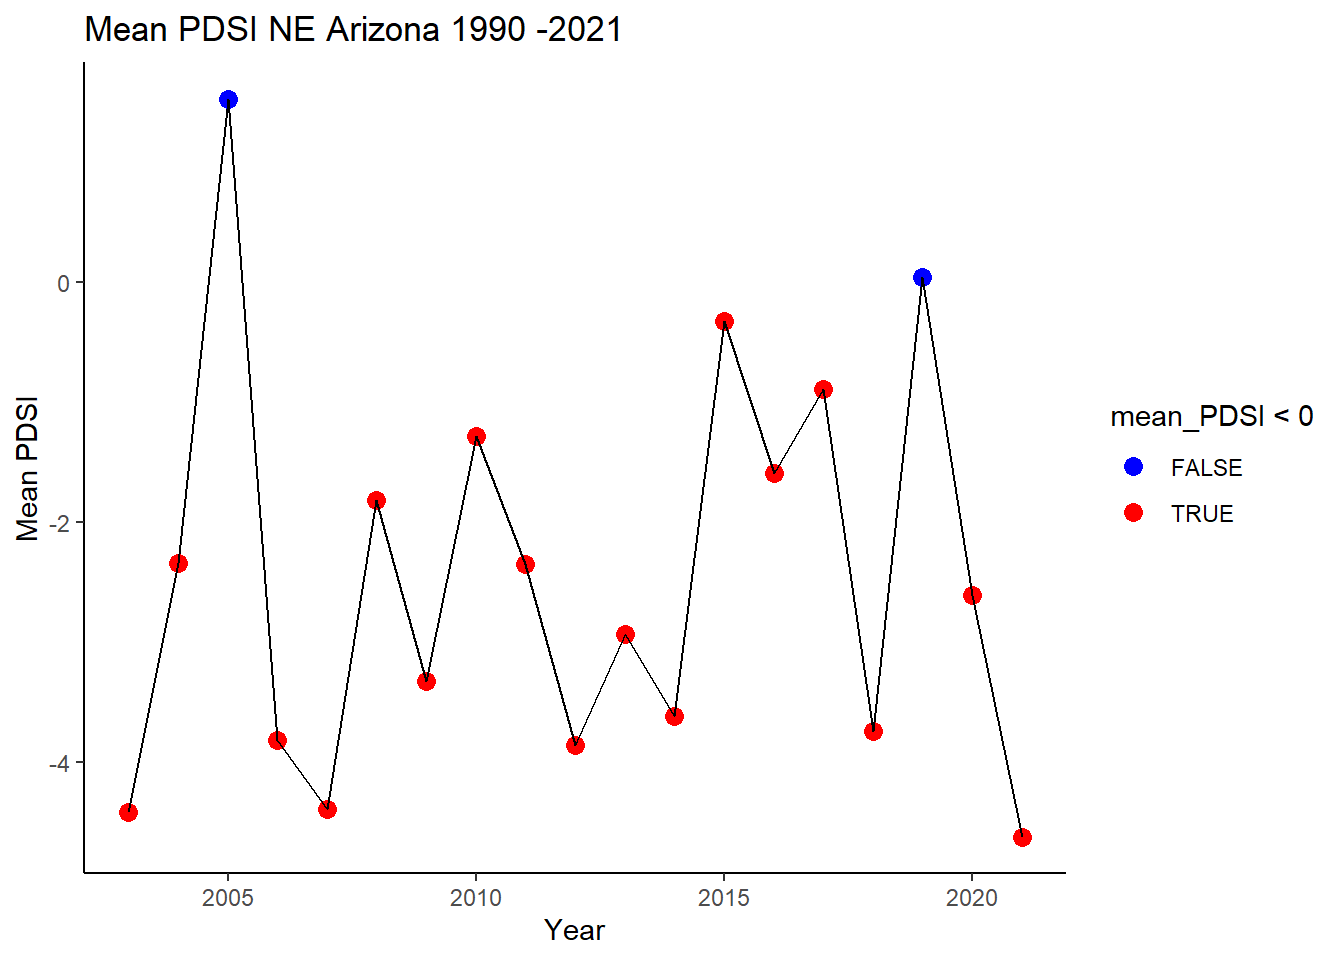
\includegraphics{ISC_6153_Assignment_2_files/figure-pdf/unnamed-chunk-12-1.pdf}

}

\end{figure}

{[}10 points{]}

\hypertarget{ecological-impact}{%
\section{Ecological impact}\label{ecological-impact}}

\textbf{(4)} How has the differential tree mortality affected the
pinyon-juniper woodland environment in Northeast Arizona? List at least
three such effects.

\textbf{Answer Q4:}

\begin{enumerate}
\def\labelenumi{\arabic{enumi}.}
\tightlist
\item
  Differential tree mortality lead to a vegetation shift in the region
  to a more Juniper dominated landscape with an age structure shift.
\item
  There was a reduction in avian seed dispersers and reproductive output
  by the system with heavier drought pressure felt on mature age classes
\item
  The differential mortality will likely alter the above and below
  ground community assemblages by altering at least avian and
  ectomycorrhizal fungi.
\end{enumerate}



\end{document}
